% HUSTthesis.tex @ https://github.com/zfengg/HUSTtex/tree/master/HUSTthesis
%
% 	A simple tex template for the undergraduate thesis at HUST.
%
% author: Zhou Feng @ 2019
%
% requirements:
%	TeX environments: TeXlive/MacTeX or MiKTeX
%	compiler: XeLaTeX
%
% ---------------------------------------------------------------------------- %
%                                   preamble                                   %
% ---------------------------------------------------------------------------- %
\documentclass[a4paper]{article}
% 10.5pt = 5 hao

% ---------------------------------- layout ---------------------------------- %
\usepackage[a4paper,top=2.5cm,bottom=2.5cm,left=3cm,right=3cm,% margins
			headheight=1.5cm,headsep=1.5em,
			footskip=2em,
			]{geometry}

% ------------------------------- math symbols ------------------------------- %
% 载入常用的数学包, 符号包
\usepackage{amsmath}
\usepackage{amsfonts}
\usepackage{amssymb}
\usepackage{mathrsfs}
\usepackage{blindtext}
\usepackage{natbib}
\setcitestyle{numbers,square}

%----------------------------------------------------------------%
%% linespace 行间距,段间距等等
\usepackage{setspace}
% \usepackage{indentfirst} % then the first line of each title should start with a indent.
% 定义标题和段落样式
% 定义1.5倍行距
\renewcommand{\baselinestretch}{1.62}
\setlength{\baselineskip}{12pt}   % set the fixed value of the lineskip
\setlength\parskip{\baselineskip} % set the space between the paragraphs, set the variable \parskip \baselineskip
% parindent
\setlength{\parindent}{0pt}

%----------------------------------------------------------------%
% fonts (style, color, size). 字体的大小,颜色,以及定义常用的字号
\usepackage{ctex}		 	% If you are lazy, the CTEX suit is enough.
% Chinese font
\usepackage{xeCJK}		 	% For the Chinese through XeLaTex
\setCJKmainfont{SimSun} 	% set the mainfont of Chinese as songti. (serif) for
\setCJKsansfont{SimSun} 	% sans serif font for \textsf
\setCJKmonofont{SimSun} 	% monospace font for \texttt
% \punctstyle{kaiming}  	% Remove the space used by symbols like comma. Special for the mainland students like us HUSTers.
\setCJKfamilyfont{song}{SimSun}                       % 宋体 song
\newcommand{\song}{\CJKfamily{song}}
\setCJKfamilyfont{kai}{KaiTi}                         % 楷体  kai
\newcommand{\kai}{\CJKfamily{kai}}
\setCJKfamilyfont{hwzs}{STZhongsong}                  % 华文中宋  hwzs
\newcommand{\hwzs}{\CJKfamily{hwzs}}
\setCJKfamilyfont{hei}{SimHei}                        % 黑体  hei
\newcommand{\hei}{\CJKfamily{hei}}
% English font
\usepackage{fontspec}% Then you can use the fonts installed at your device.
\setmainfont{Times New Roman}
\setsansfont{Times New Roman}
\setmonofont{Times New Roman}
%\setsansfont{[foo.ttf]} % for the fonts at this default path.
% font Color 利用definecolor自己可以定义颜色
\usepackage{xcolor}
\definecolor{MSBlue}{rgb}{.204,.353,.541}
\definecolor{MSLightBlue}{rgb}{.31,.506,.741}
% font Size (I use pinyin represents the corresponding size in Microsorft Word)
% \newcommand{\chuhao}{\fontsize{42pt}{\baselineskip}\selectfont}
\newcommand{\xiaochuhao}{\fontsize{36pt}{\baselineskip}\selectfont}
% \newcommand{\yihao}{\fontsize{28pt}{\baselineskip}\selectfont}
\newcommand{\erhao}{\fontsize{21pt}{\baselineskip}\selectfont}
\newcommand{\xiaoerhao}{\fontsize{18pt}{\baselineskip}\selectfont}
\newcommand{\sanhao}{\fontsize{15.75pt}{\baselineskip}\selectfont}
\newcommand{\sihao}{\fontsize{14pt}{18pt}\selectfont}
\newcommand{\xiaosihao}{\fontsize{12pt}{18pt}\selectfont}
\newcommand{\wuhao}{\fontsize{10.5pt}{18pt}\selectfont}
% \newcommand{\xiaowuhao}{\fontsize{9pt}{\baselineskip}\selectfont}
% \newcommand{\liuhao}{\fontsize{7.875pt}{\baselineskip}\selectfont}
% \newcommand{\qihao}{\fontsize{5.25pt}{\baselineskip}\selectfont}

% ---------------------------------------------------------------------------- %
%% header and footer 页眉,页脚
\usepackage{fancyhdr} % for header and footer
% 设置页眉样式
\newcommand{\headstyle}{
 \fancyhead[C]{ \hwzs\wuhao 华\hspace{0.5em}中\hspace{0.5em}科\hspace{0.5em}技\hspace{0.5em}大\hspace{0.5em}学\hspace{0.5em}毕\hspace{0.5em}业\hspace{0.5em}设\hspace{0.5em}计\hspace{0.5em}(论\hspace{0.5em}文)}
}
% 设置页脚样式
\newcommand{\footstyle}{\fancyfoot[C]{\wuhao\thepage}
 \fancyfoot[L]{\rule[5pt]{6.7cm}{0.4pt}}
 \fancyfoot[R]{\rule[5pt]{6.7cm}{0.4pt}}
}
\pagestyle{fancy}
\fancyhf{} % 清空原有样式
\headstyle
\footstyle
% 定义一种新的格式叫做main
\fancypagestyle{main}{%
 \fancyhf{} % 清空原有样式
 \headstyle
 \footstyle
}
\renewcommand{\headrulewidth}{0.4pt}
% \renewcommand{\footrulewidth}{0.4pt}
% \renewcommand{\headrule}{\rule{\textwidth}{0.4pt}}

% ---------------------------------------------------------------------------- %
% set the styles of sections at all levels
% 设置各个标题样式
% 不需要使用part和chapter层级
\usepackage{titlesec}
\usepackage{titletoc}
\titleformat{\section}{\centering\hei\bfseries\xiaoerhao}{\thesection}{1em}{} % 在section标题编号后面加个点
% \titlelabel{\thetitle.\quad} % add a dot after the counter for all levels of sections
% \titleformat*{\section}{\wuhao\bfseries} % 设置标签的形式,5号加粗
\titleformat*{\subsection}{\raggedright\hei\bfseries\sihao}
\titleformat*{\subsubsection}{\raggedright\hei\bfseries\xiaosihao}
\titleformat{\paragraph}[hang]{\raggedright\hei\bfseries\xiaosihao}{\theparagraph}{1em}{}[]

% manual
% \titleformat{command}[shape]{format}{label}{sep}{before-code}[after-code]
% \titlespacing{command}{left}{before-sep}{after-sep}
% 设置新的层级subsubsubsection
\setcounter{tocdepth}{4}
\setcounter{secnumdepth}{4}

\newcommand{\sectionbreak}{\clearpage} % 小节从新的一页开始
% 根据学校要求设置新的section, subsection, subsection,  paragraph

% set the content of section and so on
\newcommand\seccontent{
	\song
	\xiaosihao % 默认五号字体, 行间距为1.5*\baselineskip
    \setlength{\parindent}{2em} % 首段缩进两个M字符
    \setlength{\parskip}{0pt}
    }
\newcommand\tabcontent{
	\song
	\wuhao % 默认五号字体, 行间距为1.5*\baselineskip
	\setlength{\parindent}{2em} % 首段缩进两个M字符
	\setlength{\parskip}{0pt}
}


% ---------------------------------------------------------------------------- %
% for the style of theorems, definitions, proofs and remarks 定义数学里面一些常用的环境
\usepackage{amsthm}
\newtheorem{thm}{\textbf{定理}}[section]
% The section in [] can be replaced by chapter or subsection
\theoremstyle{definition} 
\theoremstyle{plain}
\theoremstyle{remark}

% ---------------------------------------------------------------------------- %
% for the caption and reference 图表及公式的编号规范
\usepackage{float} 		 		  	% table figure positioning
\usepackage{caption}
\captionsetup[figure]{labelformat=default, labelsep=quad,name={图}}
\captionsetup[table]{labelformat=default,labelsep=quad,name={表}}
% 设置图表标题的计数方式
\renewcommand{\thefigure}{\ifnum \thesection>0 \thesection-\fi \arabic{figure}} % set caption label style to 2-1
\renewcommand{\thetable}{\ifnum \thesection>0 \thesection-\fi \arabic{table}} % set caption label style to 2-1
\DeclareCaptionFont{mylabelfont}{\hei\xiaosihao}
\captionsetup[figure]{font=mylabelfont}
\captionsetup[table]{font=mylabelfont}

% 设置图表的autoref的格式
\newcommand{\reffig}[1]{图 \ref{#1}}
\newcommand{\reftab}[1]{表 \ref{#1}}
% 公式的编号格式
\renewcommand\theequation{\arabic{section}-\arabic{equation}}

\usepackage{graphicx} % To include graphixs 添加图所需的包
\usepackage{booktabs} % To create three line table including the commands toprule, bottomrule, and midrule
% \usepackage{colortbl} %
% 使用tabularx库并定义新的左右中格式
\usepackage{tabularx}
\usepackage{makecell}
\newcolumntype{L}{X}
\newcolumntype{C}{>{\centering \arraybackslash}X}
\newcolumntype{R}{>{\raggedright \arraybackslash}X}

% ---------------------------------------------------------------------------- %
% set the style of counters 设置计数器
% 设置重新计数的位置
\makeatletter
\@addtoreset{footnote}{page}
\@addtoreset{figure}{section}
\@addtoreset{table}{section}
\@addtoreset{equation}{section}
\makeatother

% ---------------------------------------------------------------------------- %
% tableofcontents, listoftables and listoffigures 目录
%\renewcommand\listfigurename{插图列表}
%\renewcommand\listtablename{表格列表}
%\titlecontents{标题名}[左间距]{标题格式}{标题标志}{无序号标题}{指引线与页码}[下间距]
%\dottedcontents{section}[2.55em]{\song \xiaosihao \bfseries}{2.5em}{1em}
\usepackage{tocloft}
\renewcommand{\contentsname}{\centerline{ \hei\bfseries\xiaoerhao 目\hspace{2em}录}}
\titlecontents{section}[3em]{\song\xiaosihao\bfseries}{\contentslabel{3em}}{\hspace*{-3em}}{\normalfont\titlerule*[8pt]{.}\contentspage}
\titlecontents{subsection}[3em]{\song\xiaosihao}{\contentslabel{3em}}{\hspace*{-3em}}{\titlerule*[8pt]{.}\contentspage}
\titlecontents{subsubsection}[4em]{\song\xiaosihao}{\contentslabel{4em}}{\hspace*{-4em}}{\titlerule*[8pt]{.}\contentspage}
\titlecontents{paragraph}[5em]{\song\xiaosihao}{\contentslabel{5em}}{\hspace*{-5em}}{\titlerule*[8pt]{.}\contentspage}

% ---------------------------------------------------------------------------- %
% reference and citation 参考文献
\usepackage{natbib}
\renewcommand{\refname}{\centering\hei\xiaoerhao 参考文献}
\bibsep=0pt % 用来设置每个\bibitem之间的间距
% \renewcommand{\bibname}{HUSTthesis} % .bib name
% \newcommand{\upcite}[1]{\textsuperscript{\textsuperscript{\cite{#1}}}} % show citation label in the upperscript

% ---------------------------------------------------------------------------- %
% 设置声明页
% 使用特殊符号
\usepackage{amssymb}
\usepackage{wasysym}
% 制作tatement中的符号
\def\HUSTcheckedbox{$\Square\!\!\!\!\checkmark$}
\def\HUSTbox{$\Square$}
% 设置命令
\newcommand{\statement}[2]{
	\def\yearofconfidentiality{\hspace{2em}}

    \def\HUSTconfidential{\HUSTbox}
	\def\HUSTnotconfidential{\HUSTcheckedbox}
	\ifnum #1<2
		\def\HUSTconfidential{\HUSTcheckedbox}
		\def\HUSTnotconfidential{\HUSTbox}
		\def\yearofconfidentiality{#2}
	\fi
	\clearpage
	\thispagestyle{main}
	\vspace*{1em}
	\seccontent
	\begin{center}
		\heiti \xiaoerhao \bfseries
		学位论文原创性声明
	\end{center}


    本人郑重声明:所呈交的论文是本人在导师的指导下独立进行研究所取得的研究成果。除了文中特别加以标注引用的内容外,本论文不包括任何其他个人或集体已经发表或撰写的成果作品。本人完全意识到本声明的法律后果由本人承担。

	\begin{flushright}
		作者签名:\hspace{6em} 年 \hspace{2em} 月 \hspace{2em} 日
	\end{flushright}
	\vspace{4em}

	\begin{center}
		\heiti \zihao{-2} \bfseries
		学位论文版权使用授权书
	\end{center}


    本学位论文作者完全了解学校有关保障、使用学位论文的规定,同意学校保留并向有关学位论文管理部门或机构送交论文的复印件和电子版,允许论文被查阅和借阅。本人授权省级优秀学士论文评选机构将本学位论文的全部或部分内容编入有关数据进行检索,可以采用影印、缩印或扫描等复制手段保存和汇编本学位论文。

    本学位论文属于 1、保密 \HUSTconfidential ,在 \yearofconfidentiality 年解密后适用本授权书。

		    \hspace{7em} 2、不保密 \HUSTnotconfidential \hspace{1em}
			。

			\hspace{7em} (请在以上相应方框内打``$\checkmark$'')



	\begin{flushright}
	作者签名:\hspace{6em} 年 \hspace{2em} 月 \hspace{2em} 日

    导师签名:\hspace{6em} 年 \hspace{2em} 月 \hspace{2em} 日
    \end{flushright}
	\clearpage
}
\newcommand{\makestatement}[2]{\statement{#1}{#2}}

% ---------------------------------------------------------------------------- %
% 定义中英文摘要和致谢环境
%
% 中文摘要环境
\newenvironment{cnabstract}[1]{
	\def \cnkeyword {#1}
	\clearpage
	\phantomsection
	\addcontentsline{toc}{section}{摘要}
	\vspace*{-20pt}
	\begin{center}
		\heiti \bfseries \xiaoerhao 摘 \hspace{2em} 要
	\end{center}
	\seccontent
}{
	\vspace{1em}
	\par\noindent {\hei\sihao \bfseries 关键词:} {\song\xiaosihao\cnkeyword}

}

% 英文摘要环境
\newenvironment{enabstract}[1]{
	\def \enkeyword {#1}
	\clearpage
	\phantomsection
	\addcontentsline{toc}{section}{Abstract}
	\vspace*{-20pt}
	\begin{center}
		\bfseries \xiaoerhao Abstract
	\end{center}
	\seccontent
}{
	\vspace{1em}
	\par\noindent {\sihao\bfseries Key Words: }\ {\song\xiaosihao\enkeyword}
	\clearpage
}

% 定义致谢环境
\newenvironment{thankpage}{
	\clearpage%
	\phantomsection%
	\addcontentsline{toc}{section}{致谢}%
	\section*{致\hspace{2em}谢}%
}{
	\clearpage
}


% ---------------------------------------------------------------------------- %
%	---	定义列表项,列举的样式
\usepackage{enumitem}
\setlist{noitemsep}

% ---------------------------------------------------------------------------- %
% \usepackage{makeindex} For the index 索引
\usepackage{listings} % For the code. 代码

% ---------------------------------------------------------------------------- %
% 设置脚注

% ---------------------------------------------------------------------------- %
%% For the hyperlink and bookmark 超链接及书签,(这样生成的pdf中的引用直接点击链接即可到达目的地)
\usepackage[bookmarks=true,colorlinks,linkcolor=black,citecolor=black,urlcolor=purple]{hyperref}% 设置超链接并修改风格


% ---------------------------------------------------------------------------- %
%% For the appendix, 附录
% 设置附录
\usepackage{appendix}
\renewcommand{\appendixname}{附录}

% ---------------------------------------------------------------------------- %
% for the titlepage 标题页,此处可以省略,建议直接使用官方给出的标题页即可
\usepackage{titling}
% 重置命令 maketitle
\renewcommand{\maketitle}{
	\def\HUSTtitlelength{12em}
 	\begin{titlepage}
		\begin{center}
			\vspace*{0em}
			
\includegraphics[height=1.61cm]{HUSTlogo.eps}\\
%
			\vspace*{4em}
%
			{\xiaochuhao \hwzs \bfseries 本科生毕业设计[论文]}\\
%
			\vspace*{6em}
			{\erhao \hei \bfseries \thetitle}

			\vspace*{6em}
			{\sanhao \hwzs
				\renewcommand\arraystretch{2.7}
				\begin{tabular}{lc}
					\makebox[4em][s]{院 \hfill 系} &
					\underline{\makebox[\HUSTtitlelength]{\school}} \\
					\makebox[4em][s]{专业班级} &
					\underline{\makebox[\HUSTtitlelength]{\classnum}} \\
					\makebox[4em][s]{姓 \hfill 名} &
					\underline{\makebox[\HUSTtitlelength]{\theauthor}} \\
					\makebox[4em][s]{学 \hfill 号} &
					\underline{\makebox[\HUSTtitlelength]{\stunum}} \\
					\makebox[4em][s]{指导教师} &
					\underline{\makebox[\HUSTtitlelength]{\instructor}} \\
			  \end{tabular}
		    }

			\vspace{4em}
			{\sanhao \hwzs \thedate}

		\end{center}
	\end{titlepage}
}

% ------------------------------------ 标题页 ----------------------------------- %
\title{毕业论文题目} % 论文题目
\def\school{电子信息与通信学院} % 院系
\def\classnum{电磁2002班} % 专业班级
\author{王锡胜舜} % 姓名
\def\stunum{U202013911}	% 学号
\def\instructor{导师姓名} % 指导老师
\date{\today} % 日期

% -------------------------------- quickinput -------------------------------- %
% 利用\newcommand{cmd}{def} 设置一些常用的代码,提高效率,这里可以自行删除,下面是我敲翻译时候打的一些command。
\newcommand{\hongzifuzhu}[1]{\textcolor{red}{\kai \wuhao(#1)}}

% ---------------------------------------------------------------------------- %
%                                   document                                   %
% ---------------------------------------------------------------------------- %
\begin{document}

\maketitle % 生成标题页,个人建议直接使用学校给的word转成pdf与这里生成的pdf第一页合并,再去打印封皮。

% \thispagestyle{empty}% 标题页不参与编号
% ------------------------------------ 声明页 ----------------------------------- %
\setcounter{page}{1}
\renewcommand{\thepage}{\Roman{page}}
\makestatement{2}{2019} % 生成声明页, 第一个参数选择1则加上保密的时间,此处为2019,如果选择2则选择不保密。

% ----------------------------------- 中文摘要 ----------------------------------- %
\setcounter{page}{1}
\renewcommand{\thepage}{\Roman{page}}
\begin{cnabstract}{$ \times\times\times\times $;$ \times\times\times\times $;$ \times\times\times\times $;$ \times\times\times\times $}
	\hspace{2em}$ \times\times\times\times\times\times\times\times\times\times\times\times\times\times\times\times\times\times\times\times\times\times\times\times\times\times\times\times\times\times\times\times\times\times\times\times\times\times\times\times\times\times\times\times\times\times\times\times\times\times\times\times\times\times\times\times\times\times\times\times\times\times\times\times\times\times\times\times\times\times\times\times\times\times\times\times\times\times\times\times\times\times\times\times\times\times\times\times\times\times\times\times\times\times\times\times\times\times\times\times\times\times\times\times\times\times\times\times\times\times\times\times\times\times\times\times\times\times\times\times\times\times\times\times\times\times\times\times\times\times\times\times\times\times\times\times\times\times\times\times\times\times\times\times\times\times\times\times\times\times\times\times\times\times\times\times\times\times\times\times\times\times\times\times\times\times\times\times\times\times\times\times\times\times\times\times\times\times\times\times\times\times\times\times\times\times\times $

	$\times\times\times\times\times\times\times\times\times\times\times\times\times\times\times\times\times\times\times\times\times\times\times\times\times\times\times\times\times\times\times\times\times\times\times\times\times\times\times\times\times\times\times\times\times\times\times\times\times\times\times\times\times\times\times\times\times\times\times\times\times\times\times\times\times\times\times\times\times\times\times\times\times\times\times\times\times\times\times\times\times\times\times\times\times\times\times\times\times\times\times\times\times\times\times\times\times\times\times\times\times\times\times\times\times\times\times\times\times\times\times\times\times\times\times\times\times\times\times\times\times\times\times\times\times\times\times\times\times\times\times\times\times\times\times\times\times\times\times\times\times\times\times\times\times\times\times\times\times\times\times\times\times\times\times\times\times\times\times\times\times\times\times\times\times\times\times\times\times\times\times\times\times\times\times\times\times\times\times\times\times\times\times\times\times\times\times $
\end{cnabstract}

% ----------------------------------- 英文摘要 ----------------------------------- %
\begin{enabstract}{$ \times\times\times\times $; $ \times\times\times\times $; $ \times\times\times\times $; $ \times\times\times\times $}

	$\times\times\times\times\times\times\times\times\times\times\times\times\times\times\times\times\times\times\times\times\times\times\times\times\times\times\times\times\times\times\times\times\times\times\times\times\times\times\times\times\times\times\times\times\times\times\times\times\times\times\times\times\times\times\times\times\times\times\times\times\times\times\times\times\times\times\times\times\times\times\times\times\times\times\times\times\times\times\times\times\times\times\times\times\times\times\times\times\times\times\times\times\times\times\times\times\times\times\times\times\times\times\times\times\times\times\times\times\times\times\times\times\times\times\times\times\times\times\times\times\times\times\times\times\times\times\times\times\times\times\times\times\times\times\times\times\times\times\times\times\times\times\times\times\times\times\times\times\times\times\times\times\times\times\times\times\times\times\times\times\times\times\times\times\times\times\times\times\times\times\times\times\times\times\times\times\times\times\times\times\times\times\times\times\times\times\times $

	$\times\times\times\times\times\times\times\times\times\times\times\times\times\times\times\times\times\times\times\times\times\times\times\times\times\times\times\times\times\times\times\times\times\times\times\times\times\times\times\times\times\times\times\times\times\times\times\times\times\times\times\times\times\times\times\times\times\times\times\times\times\times\times\times\times\times\times\times\times\times\times\times\times\times\times\times\times\times\times\times\times\times\times\times\times\times\times\times\times\times\times\times\times\times\times\times\times\times\times\times\times\times\times\times\times\times\times\times\times\times\times\times\times\times\times\times\times\times\times\times\times\times\times\times\times\times\times\times\times\times\times\times\times\times\times\times\times\times\times\times\times\times\times\times\times\times\times\times\times\times\times\times\times\times\times\times\times\times\times\times\times\times\times\times\times\times\times\times\times\times\times\times\times\times\times\times\times\times\times\times\times\times\times\times\times\times\times $
\end{enabstract}


\vspace*{-1em}
\tableofcontents
\thispagestyle{main}


\clearpage
\setcounter{page}{1}
\renewcommand{\thepage}{\arabic{page}}

% ----------------------------------- 主体内容 ----------------------------------- %
\seccontent
\section{绪论}
\hspace{12em}\hongzifuzhu{黑体小二加粗居中}

\subsection{$\times\times\times\times\times\times $}
\hongzifuzhu{黑体4号加粗,字母、阿拉伯数字为Times New Roman 4号加粗}

\subsection{$ \times\times\times\times\times\times $}
\hongzifuzhu{黑体4号加粗,字母、阿拉伯数字为Times New Roman 4号加粗}

$ \times\times\times\times\times\times\times\times\times\times\times\times\times\times\times\times\times\times\times\times\times\times\times\times\times\times\times\times\times\times\times\times\times\times\times\times\times\times\times\times\times\times\times\times\times\times\times\times\times\times\times\times\times\times\times\times\times\times\times\times\times\times\times\times\times\times\times\times\times\times\times\times\times\times\times\times\times\times\times\times\times\times\times\times\times\times\times\times\times\times\times\times\times\times\times\times\times\times\times\times\times\times\times\times\times\times\times\times\times\times\times\times\times\times\times\times\times\times\times\times\times\times\times\times\times\times\times\times\times\times\times\times\times\times\times\times\times\times\times\times\times\times\times\times\times\times\times\times\times\times\times\times\times\times\times\times\times\times\times\times\times\times\times\times\times\times\times\times\times\times\times\times\times\times\times\times\times\times\times\times\times\times\times\times\times\times\times $

\hongzifuzhu{宋体小4号, 行间距固定1.5倍行距,字符间距为标准}

\hspace{15em} \ldots\ldots\ldots

\hspace{15em} \ldots\ldots\ldots

\hspace{15em} \ldots\ldots\ldots

\subsubsection{$\times\times\times\times\times\times $}
\hongzifuzhu{黑体小4号加粗,字母、阿拉伯数字为Times New Roman 4号加粗}


\subsubsection{$\times\times\times\times\times\times $}
\hongzifuzhu{黑体小4号加粗,字母、阿拉伯数字为Times New Roman 4号加粗}

\paragraph{$ \times\times\times\times\times\times $}
\hongzifuzhu{黑体小4号加粗,字母、阿拉伯数字为Times New Roman 4号加粗}


\sectionbreak

% ---------------------------------------------------------------------------- %
\section{一级标题}
\hspace{12em}\hongzifuzhu{黑体小二加粗居中}

\subsection{二级标题}
\hongzifuzhu{黑体4号加粗,字母、阿拉伯数字为Times New Roman 4号加粗}

$ \times\times\times\times\times\times\times\times\times\times\times\times\times\times\times\times\times\times\times\times\times\times\times\times\times\times\times\times\times\times\times\times\times\times\times\times\times\times\times\times\times\times\times\times\times\times\times\times\times\times\times\times\times\times\times\times\times\times\times\times\times\times\times\times\times\times\times\times\times\times\times\times\times\times\times\times\times\times\times\times\times\times\times\times\times\times\times\times\times\times\times\times\times\times\times\times\times\times\times\times\times\times\times\times\times\times\times\times\times\times\times\times\times\times\times\times\times\times\times\times\times\times\times\times\times\times\times\times\times\times\times\times\times\times\times\times\times\times\times\times\times\times\times\times\times\times\times\times\times\times\times\times\times\times\times\times\times\times\times\times\times\times\times\times\times\times\times\times\times\times\times\times\times\times\times\times\times\times\times\times\times\times\times\times\times\times\times $

\hongzifuzhu{宋体小4号, 行间距固定1.5倍行距,字符间距为标准}

\hspace{15em} \ldots\ldots\ldots

\hspace{15em} \ldots\ldots\ldots

\hspace{15em} \ldots\ldots\ldots

\subsubsection{三级标题}
\hongzifuzhu{黑体小4号加粗,字母、阿拉伯数字为Times New Roman4号加粗}
$ \times\times\times\times\times\times\times\times\times\times\times\times\times\times\times\times\times\times\times\times\times\times\times\times\times\times\times\times\times\times\times\times\times\times\times\times\times\times\times\times\times\times\times\times\times\times\times\times\times\times\times\times\times\times\times\times\times\times\times\times\times\times\times\times\times\times\times\times\times\times\times\times\times\times\times\times\times\times\times\times\times\times\times\times\times\times\times\times\times\times\times\times\times\times\times\times\times\times\times\times $
\paragraph{四级标题}
\hongzifuzhu{黑体小4号加粗,字母、阿拉伯数字为Times New Roman4号加粗}
$ \times\times\times\times\times\times\times\times\times\times\times\times\times\times\times\times\times\times\times\times\times\times\times\times\times\times\times\times\times\times\times\times\times\times\times\times\times\times\times\times\times\times\times\times\times\times\times\times\times\times\times\times\times\times\times\times\times\times\times\times\times\times\times\times\times\times\times\times\times\times\times\times\times\times\times\times\times\times\times\times\times\times\times\times\times\times\times\times\times\times\times\times\times\times\times\times\times\times\times\times $

\sectionbreak

% ---------------------------------------------------------------------------- %
\section{方程及图表}

\hspace{12em}\hongzifuzhu{黑体小二加粗居中}

\subsection{$\times\times\times\times\times\times $}
\hongzifuzhu{黑体4号加粗,字母、阿拉伯数字为Times New Roman 4号加粗}

$ \times\times\times\times\times\times\times\times\times\times\times\times\times\times\times\times\times\times\times\times $,其 $ \times\times\times\times\times$ 可表示如下:
\begin{equation}
	E_{1}=A_{1}sin\!\left(2\pi f_{1}t+\varphi_{01}+\varphi_{path1} \right)
\end{equation}
\begin{equation}
	E_{2}=A_{2}sin\!\left(2\pi f_{2}t+\varphi_{02}+\varphi_{path2} \right)
\end{equation}

$ \times\times\times\times\times\times\times\times\times\times\times\times\times\times\times\times\times\times\times\times $  (如\reftab{table1} 所示)

\begin{table}[htpb]
	\centering
	\caption{样表}
	\label{table1}
	\song\wuhao\bfseries
	\begin{tabular}{cccc}
		\toprule
		$ \times\times\times\times\times $ & $ \times\times\times $ & $ \times\times\times $ & $ \times\times\times $ \\
		\hline
		$ \times\times\times\times\times $ & $ \times\times $       & $ \times\times $       & $ \times\times $       \\
		$ \times\times\times\times\times $ & $ \times\times $       & $ \times\times $       & $ \times\times $       \\
		$ \times\times\times\times\times $ & $ \times\times $       & $ \times\times $       & $ \times\times $       \\ 	    	\cline{2-4}
		$ \times\times\times\times\times $ & $ \times\times $       & $ \times\times $       & $ \times\times $       \\
		\bottomrule
	\end{tabular}
\end{table}
\textcolor{red}{(表标题:位于表格上方,黑体小4号,字母、阿拉伯数字为Time New Roman 小4号,表内容:宋体5号,字母、阿拉伯数字为Time New Roman 5号)\\ ``\fbox{\phantom{a}}''表示空格}

$ \times\times\times\times\times\times\times\times\times\times\times\times\times\times\times\times\times\times\times\times $  (如\reffig{testfig}所示)

\begin{figure}[H]
	\centering
	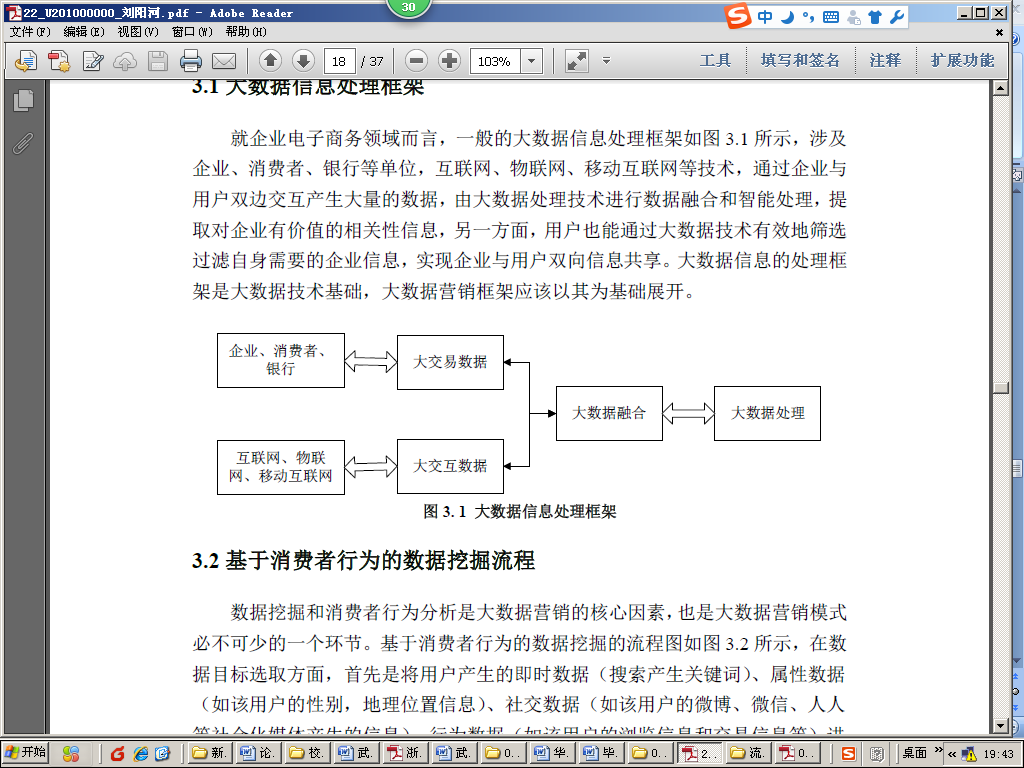
\includegraphics[width=0.75\textwidth]{testmindmap}
	\caption{测试图片, 因为学校模板给的word中的图片就是从这上面截取的部分,所以另存为PNG之后就是这个样子}
	\label{testfig}
\end{figure}
$ \times\times\times\times\times\times\times\times\times\times\times\times\times\times\times\times\times\times\times\times $  (如\reffig{E8} 所示)
\begin{figure}[H]
	\centering
	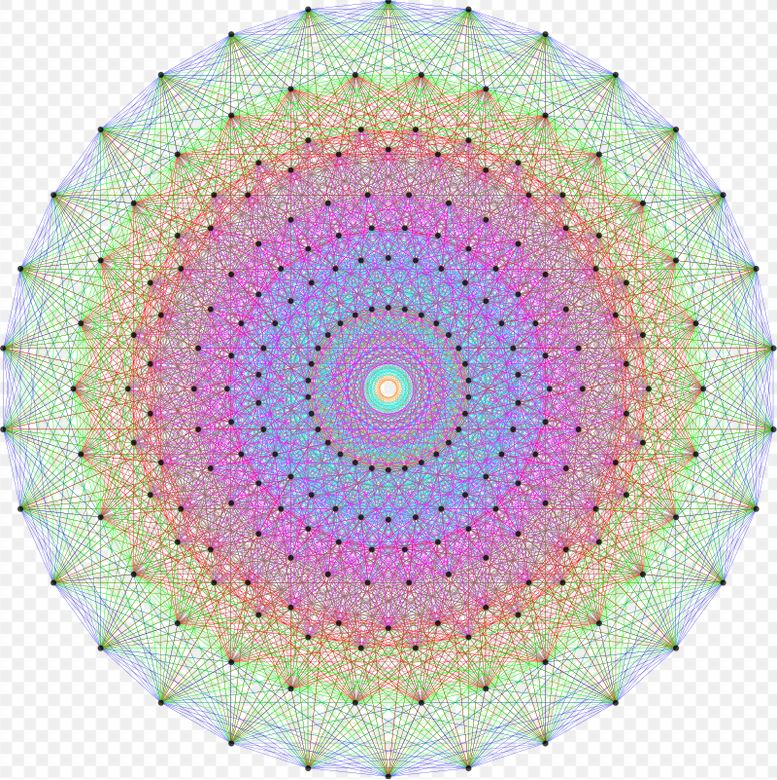
\includegraphics[width=0.5\textwidth]{E8Petrie}
	\caption{测试图片: E8 李群}
	\label{E8}
\end{figure}
\textcolor{red}{(图标题:位于图下方,黑体小4号,字母、阿拉伯数字为Time New Roman 小4号)}


\section{列举环境}
\begin{description}
	\item[列表]
	\item[枚举] \begin{enumerate}
			\item 图
			\item 表
		\end{enumerate}
	\item[列举] \begin{itemize}
			\item hello,world!

			\item 你好! \cite{Varju2018}
		\end{itemize}
\end{description}



\sectionbreak

% ---------------------------------------------------------------------------- %
\section{使用说明}\seccontent
\begin{description}
	\seccontent
	\item[基本信息] 作者:冯洲 \href{https://github.com/zfengg}{@zfengg}. 版本信息:2019/1/23, v1.0发布在 \href{https://github.com/zfengg/HUSTtex}{HUSTtex} 仓库。 如果有任何建议及纠正,欢迎 \href{https://github.com/zfengg/HUSTtex/issues}{Issue} 或者 \href{https://github.com/zfengg/HUSTtex/pulls}{Pull request}!
	
	\item[必备条件]  安装最新版本的 \href{http://www.tug.org/texlive/}{TeXLive}(推荐)或 \href{http://miktex.org/}{MiKTeX}。请确保所有宏包都更新至最新。因为中文支持利用的是包\textbf{XeCJK},所以编译器请使用 Xe\LaTeX。 编辑器推荐 \href{http://texstudio.sourceforge.net/}{TeXstudio}。 
	此文件在 Windows, Linux, MacOS 编译通过。
	
	\item[章节内部及其他环境内部的格式] 请在每个环境或章节后添加 $\backslash$seccontent (5号宋体,1.5倍行距)。 例如 
	\verb|\section\seccontent|。
	如正文中的数字和字母要加粗,Ctrl+B即可。
	
	\item[图表引用] 图标的编号及题注已设计符合要求,如要引用, 请使用$\backslash$reffig$\lbrace\rbrace$ 引用图,$\backslash$reftab$\lbrace\rbrace$引用表格,以达到要求样式。
	
	\item[公式交叉引用] 方程的编号已调好,但是引用的格式我没有另外设计,因为引用的地方可能把公式叫法不同,引用请使用自带的$\backslash$ref$\lbrace\rbrace$。
	
	\item[距离控制] 这个tex文件的距离控制可能不太精细,如果有具体的标准数值请联系,作者来完善!
	
	\item[页眉页脚] 页眉页脚的样式已经调好,距页边缘的应该也没错。如果知道精确的距离请\href{https://github.com/zfengg/HUSTtex/issues}{Issue},我马上调整,谢谢!
	\item[超链接及书签] 利用hyperref包,每个link, cite, url已调整成超链接,点击即可到达相应位置。PDF书签及链接的样式请在头文件处根据自己的喜好修改。
	
	\item[参考文献] 其实论文翻译这块给的模板并没有要求参考文献,可自行删除,但是这里提供了两种参考文献的样式:第一种使用\href{http://www.bibtex.org/}{BiB\TeX}\ 引用 \verb|.bib| 文件。第二种直接利用环境 \verb*|\thebibliography|。Tip:可以把使用BiB\TeX 生成的 \verb*|.bbl| 文件内容粘到 \verb*|.tex| 文件中以达到文件的独立性。
	
	\item[其他] 如脚标,目录,图表目录之类的,参考文献翻译没有要求,所以我就没设计,应该不会用。如果有什么特别的需要,就直接修改头文件相应内容即可。
	
	\item[注] 这个tex包含正文部分和封面部分,如果觉得这个封面不太好,那么把学校给的封面打印即可。
\end{description}


\section{随机文本测试}
\blindtext[4]


% ------------------------------------ 致谢 ------------------------------------ %
\begin{thankpage}

\end{thankpage}

% ----------------------------------- 参考文献 ----------------------------------- %
\clearpage
\phantomsection
\addcontentsline{toc}{section}{参考文献}

\bibliographystyle{plain}
\bibliography{HUSTthesis}\label{bibtexref}
\hongzifuzhu{第一个参考文献为使用 Bib\TeX 基于 $ \mathtt{HUSTthesis.bib} $ 生成。 如果不使用 Bib\TeX 可删除,然后只用后一个参考文献。}


\begin{thebibliography}{3}
	\label{latexref}
	\seccontent
	\bibitem{rudin} 王静康,张凤宝,夏淑倩等.论化工本科专业国际认证与国内认证的“实质性”.高等工程教育研究,2014,5:1-4

	\bibitem{stone} Stone J A, Howard L P. A simple technique for observing periodic nonlinearities in Michelson interferometers. Precision Engineering,1998,22(4):220-232

\end{thebibliography}

% ------------------------------------ 附录 ------------------------------------ %
\clearpage
\appendix
\phantomsection
\addcontentsline{toc}{section}{附录}
\section*{附录}


\end{document}
